\chapter{硬间隔最大化与线性可分向量机}

\textbf{Keyword: } \textsl{硬间隔最大化、软间隔最大化、核技巧}

\section{线性可分支持向量机}

\begin{define}
    (线性可分支持向量机) 给定线性可分训练数据集,通过间隔最大化成等价地求解相应的凸二次规划问题学习得到的分离
    超平面为
    \begin{equation}
        \omega^*\cdot x+b^*=0
    \end{equation}

    以及相应的分类决策函数
    \begin{equation}
        f(x)=sign( \omega^*\cdot x+b^*)
    \end{equation}

    称为\textsl{\textbf{线性可分支持向量机}}。
\end{define}

线性支持向量机假设输入空间和特征空间的元素一一对应,并将输入空间中的输入映射为特征空间中的特征向量。非线性支持
向量机利用一个从输入空间到特征孔甲你中毒非线性映射将输入映射为特征向量。所以支持向量机的学习都是在特征空间中进行的。

一般地,当训练数据集线性可分时,存在无穷个分离超平面可以将两类数据正确分开。感知机利用误分类最小策略,求得分离
超平面,不过这个时候的解有无数个。线性可分支持向量机利用\textsl{间隔最大化}求最有分离超平面,这个时候的解是唯一的。

\section{函数间隔和几何间隔}

\subsection*{函数间隔}

\begin{define}
    (函数间隔) 对于给定的训练数据集$T$和超平面$(\omega,b)$,定义超平面$(\omega,b)$关于样本点$(x_i,y_i)$
    的函数间隔为
    \begin{equation}
        \hat{\gamma}_i=y_i(\omega\cdot x_i+b)
    \end{equation}

    定义超平面$(\omega,b)$关于训练数据集$T$的函数间隔为超平面$(\omega,b)$关于$T$中所有样本点的函数间隔的最小值
    \begin{equation}
        \hat{\gamma}_i=\min\limits_{i=1,\cdots,N} \hat{\gamma}_j
    \end{equation}
\end{define}

其中点到平面的距离公式由下面的形式给出
\begin{equation}
    d=\frac{\overrightarrow{OP}\cdot \vec{n}}{\Vert \vec{n}\Vert}
\end{equation}

函数间隔可以表示分类预测的正确性和确信程度。但是选择分离超平面时,我们发现只要等比例$\omega$和$b$,分离超平面是不变的
如:
\begin{equation}
    \omega\cdot x+b=0\ \ \Leftrightarrow \ \  2\omega\cdot x+2b=0
\end{equation}

但是此时函数间隔却变成了$2$倍

\begin{equation}
    \hat{\gamma}_i=y_i(2\omega\cdot x_i+2b)=2y_i(\omega\cdot x_i+b)
\end{equation}

\subsection*{几何间隔}
因此,需要对分离超平面的法向量加某些约束,如规范化$\Vert \omega\Vert=1$,使得间隔是确定的,这时
函数间隔成为\textsl{几何间隔}。

\begin{figure}[H]
    \centering
    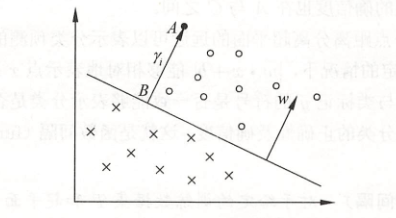
\includegraphics[scale=0.6]{figures/几何间隔.png}
    \caption{几何间隔}
\end{figure}

给定超平面$(\omega,b)$以及法向量$\omega$。点$A$表示某一实例$x_i$,分类标记为$y_i=\pm 1$。$A$与
超平面$(\omega,b)$的距离由线段$AB$给出,记为$\gamma_i$。
\begin{equation}
    \gamma_i=\pm(\frac{\omega}{\Vert \omega\Vert}\cdot x_i+\frac{b}{\Vert \omega\Vert})
\end{equation}

一般地,当样本点$(x_i,y_i)$被正确分类时,点$x_i$与超平面$(\omega,b)$的距离为
\begin{equation}
    \gamma_i=y_i(\frac{\omega}{\Vert \omega\Vert}\cdot x_i+\frac{b}{\Vert \omega\Vert})
\end{equation}

\begin{define}
    (几何间隔) 对于给定的训练数据集$T$和超平面$(\omega,b)$,定义超平面$(\omega,b)$关于样本点$(x_i,y_i)$
    的几何间隔为
    \begin{equation}
        \gamma_i=y_i(\frac{\omega}{\Vert \omega\Vert}\cdot x_i+\frac{b}{\Vert \omega\Vert})
    \end{equation}

    定义超平面$(\omega,b)$关于训练数据集$T$的几何间隔为超平面$(\omega,b)$关于$T$中所有样本点的几何间隔的最小值
    \begin{equation}
        \gamma_i=\min\limits_{i=1,\cdots,N} \hat{\gamma}_j
    \end{equation}
\end{define}

\subsection*{函数间隔和几何间隔的关系}

从函数间隔和几何间隔的定义,二者有如下关系
\begin{equation}
    \gamma=\frac{\hat{\gamma}}{\Vert \omega\Vert}
\end{equation}

可见如果$\Vert \omega\Vert=1$,则二者相等。如果超平面参数$\omega$和$b$成比例改变,函数间隔也成比例改变而几何间隔不变。

\section{最大间隔分离超平面}

如何求得几何间隔最大的分离超平面?这个问题表述为下列优化问题
\begin{equation}
    \begin{aligned}
    &\max\limits_{\omega,b}\ \ \gamma\\
    &s.t.\ \ \ \ y_i(\frac{\omega}{\Vert \omega\Vert}\cdot x_i+\frac{b}{
        \Vert \omega\Vert})\geqslant \gamma,\ \ \ i=1,2,\cdots,N
\end{aligned}
\end{equation}

考虑几何间隔和函数间隔的关系,优化问题等价为
\begin{equation}
    \begin{aligned}
    &\max\limits_{\omega,b}\ \ \frac{\hat{\gamma}}{\Vert \omega\Vert}\\
    &s.t.\ \ \ \ y_i(\frac{\omega}{\Vert \omega\Vert}\cdot x_i+\frac{b}{
        \Vert \omega\Vert})\geqslant \hat{\gamma},\ \ \ i=1,2,\cdots,N
\end{aligned}
\end{equation}

函数间隔$\hat{\gamma}$的取值并不影响优化问题的解。事实上,假设$\omega$和$b$成比例改变为
$\lambda\omega$和$\lambda b$,这时函数间隔成为$\lambda \hat{r}$。函数间隔的这一改变
对上面最优化问题的不等式约束没有影响,对目标函数的优化也没有影响,即它产生一个等价的最优化问题,
这样就可以取$\hat{\gamma}=1$代入优化问题。

\subsection*{等价的优化问题}
注意到最大化$1/\Vert\omega\Vert$和最小化$\frac{1}{2}\Vert\omega\Vert^2$
是等价的\footnote{在趋近于$0$时,$\frac{1}{2}\Vert\omega\Vert^2$趋于最小,而$\frac{1}{\Vert\omega\Vert}$趋于最大}。
于是就得到下面的线性可分支持向量机学习的最优化问题:
\begin{framed}
\begin{equation}
    \begin{aligned}
    &\max\limits_{\omega,b}\ \ \frac{1}{2}\Vert\omega\Vert^2\\
    &s.t.\ \ \ \ y_i(\frac{\omega}{\Vert \omega\Vert}\cdot x_i+\frac{b}{
        \Vert \omega\Vert})\geqslant 1,\ \ \ i=1,2,\cdots,N
\end{aligned}
\end{equation}
\end{framed}

这是一个\textsl{凸二次规划问题}。通俗来描述这个问题是,寻找到一个超平面,使得样本数据集到超平面的
几何间距最大,但同时几何间距又收到本身定义的制约,即样本数据集的几何间距是所有样本点几何间距的最小值。

\section{最大间隔算法}
输入:线性可分训练数据集$T=\{(x_1,y_1),(x_2,y_2),\cdots,(x_N,y_N)\}$,其中$x_i\in \mathbb{R}^n$,
$y_i\in \{-1,+1\}$。

输出:最大间隔分离超平面和分类决策函数。

\begin{enumerate}[itemindent=2em]
    \item 构造并求解约束最优化问题
    \begin{equation}
        \begin{aligned}
            & \min\limits_{\omega,b}\ \frac{1}{2}\Vert \omega\Vert^2\\
            & s.t. \ \ y_i(\omega\cdot x_i+b)-1\geqslant 0,\ \ i=1,2,\cdots,N
        \end{aligned}
    \end{equation}

    求得最优解$\omega^*,b^*$。
    \item 由此得到分离超平面
    \begin{equation}
        \omega^*\cdot x+b^*=0
    \end{equation}

    分类决策函数可以写成
    \begin{equation}
        f(x)=sign(\omega^*\cdot x+b^*)
    \end{equation}
\end{enumerate}

\section{最大间隔超平面的存在性和唯一性}
\begin{theorem}
    若训练数据集$T$是线性可分的,则可将数据集中样本点完全正确分开的最大间隔分离超平面存在且唯一
\end{theorem}
\textbf{proof. } 


\section{支持向量和间隔边界}

训练数据集的样本点中与分离超平面距离最近的样本点的实例称为\textsl{\textbf{支持向量}(support vector)}。
支持向量是使得约束条件$y_i(\frac{\omega}{\Vert \omega\Vert}\cdot x_i+\frac{b}{
    \Vert \omega\Vert})\geqslant \gamma_i,\ \ \ i=1,2,\cdots,N$成立的点,即
    \begin{equation}
        y_i(\omega\cdot x_i+b)-1=0
    \end{equation}

    对于$y_1=+1$的正例点,支持向量在超平面
    \begin{equation}
        H_1:\omega\cdot x+b=1
    \end{equation}

    对于$y_1=-1$的服例点,支持向量在超平面
    \begin{equation}
        H_2:\omega\cdot x+b=-1
    \end{equation}

如下图所示,$H_1$和$H_2$上的点就是支持向量。

\begin{figure}[H]
    \centering
    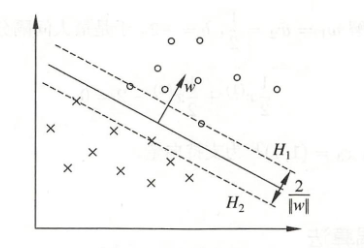
\includegraphics[scale=0.6]{figures/支持向量.png}
    \caption{支持向量}
\end{figure}

$H_1$和$H_2$之间的距离称为\textsl{\textbf{间隔}(margin)}。间隔依赖于分离超平面的法向量$\omega$,
等于$2/\Vert\omega\Vert$。$H_1$和$H_2$称为\textsl{\textbf{间隔边界}(margin boundary)}。

在决定分离超平面时,只有支持向量起作用,而其他实例点不起作用。所以支持向量机由很少的
支持向量作为训练样本决定。

%对偶算法
\section{支持向量机的对偶算法}

应用\textsl{\textbf{拉格朗日对偶性}},通过求解\textsl{\textbf{对偶问题}(dual problem)}得到原始问题
的最优解。这就是线性可分支持向量机的对偶算法。

首先构建\textsl{\textbf{拉格朗日函数}(Lagrange function)}。引入\textsl{\textbf{拉格朗日乘子}
(Lagrange multiplier)}:$\alpha_1\geqslant 0$。
\begin{equation}
    L(\omega,b,\alpha_i)=\frac{1}{2}\Vert\omega\Vert^2-\sum\limits_{i=1}^{N}\alpha_i
    y_i(\omega\cdot x_i+b)+\sum\limits_{i=1}^{N}\alpha_i
\end{equation}

其中$\alpha=(\alpha_1,\alpha_2,\cdots,\alpha_N)^T$为拉格朗日乘子向量。根据拉格朗日乘子法,
原始问题的对偶问题是极大极小问题
\begin{equation}
    \max\limits_{\alpha}\min\limits_{\omega,b}L(\omega,b,\alpha)
    \label{对偶最优化问题}
\end{equation}

\begin{theorem}
    设$\alpha^*=(\alpha^*_1,\alpha^*_2,\cdots,\alpha^*_l)^T$是最优化对偶问题(\ref{对偶最优化问题})
    的解,则存在下标$j$,使得$\alpha^*_j>0$,并可按照下式求得原始最优化问题的解$\omega^*,b^*$。
    \begin{equation}
        \omega^*=\sum\limits_{i=1}^{N}\alpha^*_iy_ix_i
    \end{equation}
    \begin{equation}
        b^*=y_i-\sum\limits_{i=1}^{N}\alpha^*_iy_i(x_i\cdot x_j)
    \end{equation}
\end{theorem}

由此定理,分离超平面可以写成
\begin{equation}
    \sum\limits_{i=1}^{N}\alpha^*_iy_i(x\cdot x_i)+b^*=0
\end{equation}
分类决策函数可以写成
\begin{equation}
    f(x)=sign(\sum\limits_{i=1}^{N}\alpha^*_iy_i(x\cdot x_i)+b^*)
\end{equation}

这样分类决策函数只依赖于输入$x$和训练样本输入的内积。$f(x)=sign(\sum\limits_{i=1}^{N}\alpha^*_iy_i(x\cdot x_i)+b^*)$
\textsl{\textbf{线性可分支持向量机的对偶形式}}。

\subsection*{线性可分支持向量机学习算法}

输入:线性可分训练集$T={(x_1,,y_1),(x_2,y_2),\cdots,(x_N,y_N)}$,其中$x_i\in \mathbb{R}^n$,$y_i\in \{-1,+1\}$。
输出:分离超平面和分类决策函数

\begin{enumerate}
    \item 构造并求解约束最优化问题
    \begin{equation}
        \begin{aligned}
            & \min\limits_{\alpha} \frac{1}{2}\sum\limits_{i=1}^{N}\sum\limits_{j=1}^{N}
            \alpha_i\alpha_jy_iy_j(x_i\cdot x_j)=\sum\limits_{i=1}^{N}\alpha_i\\
            &.s.t \sum\limits_{i=1}^{N}\alpha_iy_i=0\\
            & \ \ \ \ \ \alpha_i\geqslant 0,\ \ \ i=1,2,\cdots,N
        \end{aligned}
    \end{equation}
    
    求得最优解$\alpha^*=(\alpha^*_1,\alpha^*_2,\cdots,\alpha^*_N)^T$
    \item 计算
    \begin{equation}
        \omega^*=\sum\limits_{i=0}^{N} \alpha^*_i y_i x_i
    \end{equation}

    并选择$\alpha^*$的一个正分量$\alpha^*_j>0$计算
    \begin{equation}
        b^*=y_i\sum\limits_{i=1}^{N}\alpha^*_iy_i(x_i\cdot x_j)
    \end{equation}
    \item 求得分离超平面和决策函数
    \begin{equation}
        \omega^*\cdot x+b^*=0
    \end{equation}
    \begin{equation}
        f(x)=sign(\omega^*\cdot x+b^*)
    \end{equation}
\end{enumerate}



线性可分支持向量机中,$\omega^*$和$b^*$只依赖于训练数据中对应$\alpha^*_i>0$的样本点$(x_i,y_i)$,我们将
训练数据中对应于$\alpha^*_i>0$的实例点$x_I\in \mathbb{R}^n$称为支持向量。

\begin{define}[支持向量]
    考虑原始最优化问题以及对偶最优化问题,将训练数据集集中对应于$\alpha^*_i>0$的样本点$(x_i,y_i)$的实例
    $x_i\in \mathbb{R}^n$称为\textsl{\textbf{支持向量}}。
\end{define}